\documentclass[12pt]{beamer}

\hypersetup{colorlinks=true,linkcolor=red}
\usetheme{default}
\usecolortheme{albatross}

\usepackage[utf8]{inputenc}
\usepackage[russian,english]{babel}
\usepackage[T2A]{fontenc}
\usepackage{hyperref}
\usepackage[final]{listings}
\usepackage{breakurl}
\usepackage{cite}
\usepackage{perpage}

\graphicspath{{img/}}

\def\Url\Breaks{\do\/\do-}
\lstset{
  frame=single,
  breaklines=true,
  basicstyle=\tiny,
  postbreak=\raisebox{0ex}{\ensuremath{\hookrightarrow\space}},
  numbers=left
}

\lstdefinestyle{base}{
  frame=single,
  breaklines=true,
  basicstyle=\tiny,
  postbreak=\raisebox{0ex}{\ensuremath{\hookrightarrow\space}},
  moredelim=[is][\color{red}]{@}{@},
  numbers=left
}

\MakePerPage{footnote}

\title{Operating Systems}
\subtitle{File Systems}
\author{Me}
\date{\today}

\begin{document}
  \begin{frame}
    \titlepage
  \end{frame}

  \begin{frame}
\frametitle{Файловая система}
\begin{itemize}
  \item Блочные устройства позволяют хранить большие объемы информации долгое
  время
  \begin{itemize}
    \item чем больше информации тем больше хочется ее структурировать.
  \end{itemize}
  \item Multics впервые (*) ввел в использование иерархическую файловую систему:
  \begin{itemize}
    \item файлы, каталоги/директории/папки, жесткие и символьные ссылки;
    \item так как Multics пофейлился, популярной иерархиеские ФС сделал скорее
    Unix.
  \end{itemize}
\end{itemize}
\end{frame}

\begin{frame}
\frametitle{Операции над файлами}
\begin{itemize}
  \item открытие файла - возвращает некоторый дескриптор, который используется
  для дальнейших операций с файлами
  \begin{itemize}
    \item снаружи этот дескриптор обычно выглядит просто как целое число;
    \item внутри ОС это обычно некоторая структура, которая кеширует информацию
    о файле (размер, права доступа, дата модификации и тд и тп);
  \end{itemize}
  \item закрытие файла - освобождение всех ресурсов связанных с открытым
  файлом;
  \item чтение и запись по некоторому смещеную в файле;
  \item запись за пределы файла изменяет его размер.
\end{itemize}
\end{frame}

\begin{frame}
\frametitle{Операции над каталогами}
\begin{itemize}
  \item создание и удаление файлов/жестких ссылок на файлы;
  \item создание и удаление символьных ссылок на файлы и каталоги;
  \item создание и удаление других каталогов;
  \item перечисление файлов/каталогов внутри каталогов.
\end{itemize}
\end{frame}

  \begin{frame}
\frametitle{Простейшая файловая система}
\begin{itemize}
  \item Основная структура данных - связный список:
  \begin{itemize}
    \item мы будем связывать в список блоки фиксированного размера;
    \item размер блока кратен размеру сектора диска.
  \end{itemize}
  \item Файлы
  \begin{itemize}
    \item файл идентифицируется первым блоком;
    \item все блоки с содержимым файла просто связаны в список.
  \end{itemize}
  \item Каталоги
  \begin{itemize}
    \item каталог - файл, который хранит записи фиксированного формата
    \begin{itemize}
      \item каждая запись хранит имя дочернего каталога/файла, тип и номер
      первого блока.
    \end{itemize}
  \end{itemize}
  \item Свободные блоки
  \begin{itemize}
    \item все свободные блоки просто связаны в список.
  \end{itemize}
\end{itemize}
\end{frame}

\begin{frame}
\frametitle{"Эффективный" связный список}
\begin{itemize}
  \item Связный список не очень эффективная структура данных для индексации
  \begin{itemize}
    \item но мы все же постараемся сделать с этим что-нибудь...
    \item ну хоть что-нибудь...
  \end{itemize}
  \item Что нужно учитывать?
  \begin{itemize}
    \item общение с диском осуществляется секторами (минимум 512 байт);
    \item общение с диском медленное - чем меньше обращений тем лучше.
  \end{itemize}
\end{itemize}
\end{frame}

\begin{frame}
\frametitle{"Эффективный" связный список}
\begin{itemize}
  \item Заведем таблицу:
  \begin{itemize}
    \item каждая запись в таблице соответствует блоку ФС (i-ая запись,
    соответствует i-ому блоку);
    \item каждая запись - это просто число, а именно номер следующего блока или
    маркер конца списка.
  \end{itemize}
  \item Почему не хранить ссылку на следующий блок прямо в блоке?
  \begin{itemize}
    \item таблица гораздо компактнее - за одно чтение мы получаем сразу
    несколько ссылок;
    \item если повезет, то это будут нужные нам ссылки;
    \item если повезет, то мы можем прочитать всю таблицу целиком и хранить ее
    в памяти.
  \end{itemize}
\end{itemize}
\end{frame}

\begin{frame}
\frametitle{File Allocation Table (FAT)}
\begin{itemize}
  \item ФС FAT12/16/32 - пожалуй одна из самых популярных ФС в мире:
  \begin{itemize}
    \item активно используется во всяких устройствах (MP3 плееры, фотоаппараты,
    USB флешки и т.д. и т.п.);
    \item мало функциональная;
    \item не очень надежная;
    \item зато очень простая.
  \end{itemize}
  \item FAT использует связные списки и похожую таблицу блоков
  \begin{itemize}
    \item эта таблица и называется File Allocation Table (FAT).
  \end{itemize}
\end{itemize}
\end{frame}

  \begin{frame}
\frametitle{Суперблок}
\begin{itemize}
  \item ФС начинается с суперблока
  \begin{itemize}
    \item суперблок - это структура, которая хранит общую информацию о ФС
    \begin{itemize}
      \item магическое число/строка - чтобы убедиться, что на диске хранится
      именно наша ФС;
      \item размер блока ФС;
      \item версия ФС;
      \item ссылки на какие-то общие структуры ФС, например, список свободных
      блоков.
    \end{itemize}
    \item Суперблок хранится в каком-то известном месте диска
    \begin{itemize}
      \item иногда на диске хранится несколько копий супеблока, чтобы если один
      из них испортится, то можно будет использовать другой;
      \item потеря суперблока, это практически потеря ФС.
    \end{itemize}
  \end{itemize}
\end{itemize}
\end{frame}

\begin{frame}
\frametitle{Индексные узлы (Inode-ы)}
\begin{itemize}
  \item Inode - важная структура в классических Unix-овых (и не только) ФС
  \begin{itemize}
    \item Inode пресдтавляет сущность внутри ФС (файл/каталог):
    \begin{itemize}
      \item хранит права/привелегии доступа, даты модификации и прочее;
      \item размер файла/каталога и \emph{раcположение его блоков на диске};
      \item примерное представление об содержимом Inode вам может дать
      \emph{man 2 stat};
    \end{itemize}
    \item каждый Inode имеет уникальный идентификатор, по которому его можно
    найти на диске
    \begin{itemize}
      \item зная идентификатор вы можете легко найти Inode на диске;
      \item в классических ФС, при форматировании выделяется таблица Inode-ов;
      \item идентификатор Inode - это просто его позиция в таблице.
    \end{itemize}
  \end{itemize}
\end{itemize}
\end{frame}

\begin{frame}
\frametitle{Описание расположения блоков}
\begin{center}
  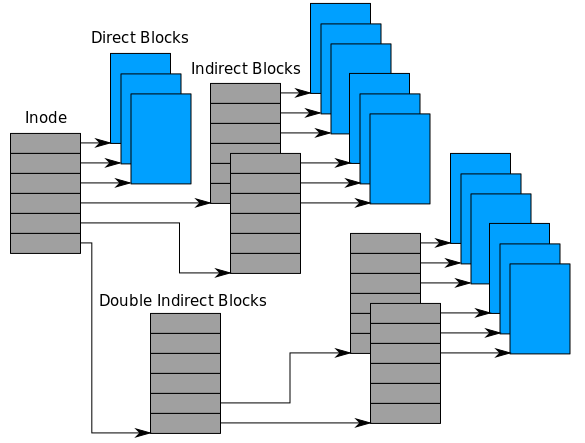
\includegraphics[width=.8\linewidth]{inode.png}
\end{center}
\end{frame}

\begin{frame}
\frametitle{Fast File System}
\begin{itemize}
  \item Fast File System - первая из классических Unix-овых ФС, в которой были
  учтены особенности диска
  \begin{itemize}
    \item не то, чтобы до этого никто не заботился о производительности;
    \item но ребята из Berkely, которые создали FFS довольно буедительно
    показали, что диск в ФС того времени использовался неэффективно.
  \end{itemize}
  \item В Fast File System минимальный размер блока - 4Kb
  \begin{itemize}
    \item т. е. за одно обращение к диску ФС пишет/читаете сразу 8 секторов;
    \item это привело к заметному увеличению скорости работы ФС, что ясно
    показало, что другими ФС диск использовался не эффективно.
  \end{itemize}
\end{itemize}
\end{frame}

\begin{frame}
\frametitle{Цилиндровые группы}
\begin{itemize}
  \item Цилиндровая группа - группа блоков, которые расположены на диске рядом
  \begin{itemize}
    \item цилиндровые группы - еще одна оптимизация введенная в FFS;
    \item каждая цилиндровая группа содержит свой набор Inode-ов, битовую карту
    свободных/занятых блоков внутри группы и прочее.
  \end{itemize}
  \item Цилиндровые группы используются для более эффективной аллокации ресурсов
  на диске:
  \begin{itemize}
    \item достаточно большие куски файла пытаются положить в одну цилиндровую
    группу;
    \item Inode-ы файлов в одном каталоге, стараются также положить в одну
    цилиндровую группу;
    \item при этом стараемся не заполнять цилинддровые группы под завязку.
  \end{itemize}
\end{itemize}
\end{frame}

\begin{frame}
\frametitle{Классические Unix-овые ФС}
\begin{itemize}
  \item FFS - это предшественник классических Unix-овых ФС
  \begin{itemize}
    \item сейчас никто не использует FFS (скорее всего), но многие пользуются
    ее наследниками: ext3 и ext4 (ext2, если кто-то ей пользуется).
  \end{itemize}
  \item Многие детали отличаются, но многие идеи остаются:
  \begin{itemize}
    \item например, каталог это не просто набор записей, а HTree/B+-tree или
    какая-то подобная индексная структура данных;
    \item журналирование для обеспечения консистентности вместо soft updates;
    \item а цилиндровые группы остались, хотя возможно называются по-другому.
  \end{itemize}
\end{itemize}
\end{frame}

  \begin{frame}
\frametitle{Индексные структуры данных}
\begin{itemize}
  \item Для быстрого поиска файла/каталога внутри каталога или смещения на диске
  по смещению внутри файла можно использовать подходящую структуру данных:
  \begin{itemize}
    \item чтобы быстро находить и открывать файлы по имени;
    \item чтобы читать/писать файлы не по-порядку.
  \end{itemize}
  \item Имя подхоядщий словарь мы вообще можем хранить все дерево каталогов в
  одном словаре:
  \begin{itemize}
    \item отображаем номер Inode родительского каталога и имя на номер Inode
    файла/каталога внутри каталога;
    \item с таким словарем нам даже не нужно заранее выделять место под таблицу
    Inode-ов - мы можем просто хранить их в таком словаре.
  \end{itemize}
\end{itemize}
\end{frame}

\begin{frame}
\frametitle{Деревья поиска}
\begin{itemize}
  \item Бинарные деревья поиска - классический вариант индексной структуры
  данных в памяти:
  \begin{itemize}
    \item Red-Black деревья;
    \item AVL деревья;
    \item Splay деревья;
    \item декартовы деревья.
  \end{itemize}
  \item Бинарные деревья поиска не годятся в качестве индекса на диске
  \begin{itemize}
    \item они неэффективны для блочного интерфейса (меньше 512 байт за раз
    читать/писать мы все равно не можем);
    \item бинарные деревья поиска очень высокие (даже идеально
    сбалансированные).
  \end{itemize}
\end{itemize}
\end{frame}

\begin{frame}
\frametitle{Ветвистые деревья}
\begin{itemize}
  \item Если бинарные деревья поиска слишком высокие, то просто будем
  использовать N-арные, где N будет 10, 100, 1000...
  \begin{itemize}
    \item если каждый узел может хранить больше 2 ссылок на дочерние узлы, то
    высота дерева может быть меньше;
    \item за одно обращение к диску мы можем читать сразу N ссылок.
  \end{itemize}
  \item $B$-деревья - идеально сбалансированные N-арные деревья поиска:
  \begin{itemize}
    \item со временем $B$-деревья получили много вариаций: $B+$, $B^*$,
    $B^\epsilon$;
    \item вариации $B$-деревьев используются повсеместно для индексации (в ФС,
    базах данных, Key-Value Store-ах и прочих).
  \end{itemize}
\end{itemize}
\end{frame}

  \begin{frame}
\frametitle{B+ деревья}
\begin{itemize}
  \item B+ дерево - идеально сбалансированное сильно ветвистое дерево
  поиска, которое хранит значения только в листьях:
  \begin{itemize}
    \item растояние от корня до всех листьев одинаковое;
    \item каждый узел кроме корня хранит не менее B ключей, где B
    некоторый фиксированный параметр дерева;
    \item словарь хранит пары - (ключ, значение) - все внутренние узлы
    хранят только ключи, и только листья хранят полные пары.
  \end{itemize}
\end{itemize}
\end{frame}

\begin{frame}
\frametitle{Реализации B+ деревьев}
\begin{itemize}
  \item Есть много подходов к реализации B+ деревьев и, соответсвенно, к
  балансировке
  \begin{itemize}
    \item мы рассмотрим классический вариант B+ деревьев с балансировкой
    снизу вверх;
    \item а также то, что называется COW B+ деревья - это самый простой
    вариант;
    \item COW B+ деревья реально используются на практике в ФС Btrfs.
  \end{itemize}
\end{itemize}
\end{frame}

\begin{frame}
\frametitle{Узел B+ дерева}
\begin{center}
  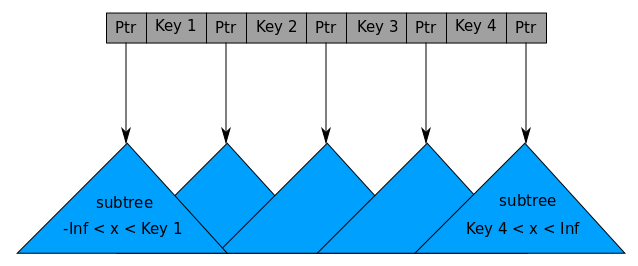
\includegraphics[width=.6\linewidth]{bnode.png}
\end{center}
\begin{itemize}
  \item Каждый узел хранит от $B$ до $2B$ ключей и ссылок на следущие узлы:
  \begin{itemize}
    \item корень - исключение, он может хранить произвольное количество
    ключей и ссылок на следующие узлы;
    \item листья не хранят ссылки на следующие узлы;
    \item ограничение весьма условно, не редко границы делают шире: $B$ и
    $4B$, чтобы обеспечить гистерезис.
  \end{itemize}
\end{itemize}
\end{frame}

\begin{frame}
\frametitle{Поиск в B+ дереве}
\begin{itemize}
  \item Поиск в B+ дереве похож на поиск в бинарном дереве поиска:
  \begin{itemize}
    \item что не удивительно, ведь B+ дерево тоже является деревом поиска;
    \item на каждом шаге просто выбираем поддерево, в котором может
    содержаться нужный ключ и повторяем поиск рекурсивно, пока не дойдем до
    листа.
  \end{itemize}
  \item Сложность поиска:
  \begin{itemize}
    \item для нас в первую очередь важны операции обращения к диску - чтения
    и записи узлов дерева;
    \item количество чтений - высота дерева;
    \item все узлы кроме, возможно, корня, содержат как миниум $B$ ключей;
    \item высота дерева ограничена снизу как $1 + log_B N$, где $N$ -
    количество пар в дереве.
  \end{itemize}
\end{itemize}
\end{frame}

\begin{frame}
\frametitle{Вставка в B+ дерево}
\begin{itemize}
  \item Вставка в целом протекает так же как и поиск:
  \begin{itemize}
    \item на каждом шаге мы выбираем поддерево, в которой должен попасть
    новый ключ;
    \item но вставка может изменить количество ключей, а значит может
    нарушить ограничения на количество ключей в узле дерева - и нам придется
    это исправлять.
  \end{itemize}
  \item Допустим мы нашли нужный лист, у нас может быть два варианта:
  \begin{itemize}
    \item в листе достаточно места для нового ключа - перебалансировка не
    потребуется требуется;
    \item в листе не достаточно места - нам нужно разбить узел на два и
    поделить все ключи, включая новый, между двумя новыми узлами поровну.
  \end{itemize}
\end{itemize}
\end{frame}

\begin{frame}
\frametitle{Вставка в B+ дерево}
\begin{itemize}
  \item Если нам пришлось разбить лист на два новых узла, то нам нужно
  обновить родителя, здесь возможны несколько враинтов:
  \begin{itemize}
    \item родителя нет, а лист так же является корнем - в этом случае нужно
    создать новый пустой узел и добавить в него ссылки на два созданных узла,
    он станет новым корнем дерева;
    \item родитель сам полон и в него уже нельзя добавить ключ - в этом
    случае мы можем разбить родителя на два узла, как мы делали это с листом
    и повторить операцию рекурсивно;
    \item в родителе достаточно места для нового ключа - перебалансировка не
    требуется.
  \end{itemize}
\end{itemize}
\end{frame}

\begin{frame}
\frametitle{Удаление из B+ дерева}
\begin{itemize}
  \item Как и со вставкой для начала найдем нужный лист и нужный ключ в
  листе, далее возможны два варианта:
  \begin{itemize}
    \item в узле даже после удаление достаточно ключей - перебалансировка
    не требуется;
    \item после удаления в кзле слишком мало ключей - потребуется
    перебалансировка, возможно.
  \end{itemize}
\end{itemize}
\end{frame}

\begin{frame}
\frametitle{Удаление из B+ дерева}
\begin{itemize}
  \item Итак в узле слишком мало ключей, у нас есть несколько возможностей:
  \begin{itemize}
    \item у узла есть левый/правый брат:
    \begin{itemize}
      \item суммарно в узле и его брате достаточно ключей на два узла, то
      их можно перераспределить и обновить ключи в родительском узле;
      \item суммарно в узле и его брате не достаточно ключей на два узла,
      тогда их нужно их объединить, при этом из родителя придется удалить
      один ключ;
    \end{itemize}
    \item у узла нет братьев, а значит наш узел - корень дерева, и тут
    возможны варианты:
    \begin{itemize}
      \item в корне осталась только одна ссылка на дочерний узел - мы можем
      просто удалить этот корень и заменить его ребенком;
      \item в корне осталось больше одной ссылки - никаких модификаций не
      требуется.
    \end{itemize}
  \end{itemize}
\end{itemize}
\end{frame}

\begin{frame}
\frametitle{COW B+ дерево}
\begin{itemize}
  \item В рассмотренном ранее варианте мы сначала искали нужный лист для
  вставки/удаления, а затем двигаясь от листьев к корню восстанавливали
  инварианты дерева
  \begin{itemize}
    \item но можно во время поиска нужного листа сразу исправлять дерево
    так, чтобы инварианты не нарушались при вставке/удалениию.
  \end{itemize}
  \item Вставка:
  \begin{itemize}
    \item если при поиске нужного листа мы натыкаемся на полный узел,
    вставка в который, приведет к разбиению, то мы разбиваем его заранее
    по мере прохода вниз по дереву.
  \end{itemize}
  \item Удаление:
  \begin{itemize}
    \item аналогично вставке, но теперь мы перебалансируем если находим
    узел с малым числом ключей, при этом требуется особенная забота о
    корне.
  \end{itemize}
\end{itemize}
\end{frame}

  \begin{frame}
\frametitle{Log-Structured Merge Tree (LSM)}
\begin{itemize}
  \item Недостатки B+ деревьев:
  \begin{itemize}
    \item вставка и удаление в/из B+ дерева сложные;
    \item параллельная работа с B+ деревьями сложная.
  \end{itemize}
  \item Можно сделать проще:
  \begin{itemize}
    \item пожертвовав алгоритмической сложностью поиска;
    \item получив в замен "эффективную" параллельную работу.
  \end{itemize}
\end{itemize}
\end{frame}

\begin{frame}
\frametitle{Нам понадобятся}
\begin{itemize}
  \item Упорядоченный словарь в памяти с операцией вставки:
  \begin{itemize}
    \item если ключ уже есть в словаре, то нужно заменить занчение;
    \item подойдет любое дерево поиска, но плохо для параллельной обработки;
    \item популярный вариант Skiplist - сравнительно легко параллелится.
  \end{itemize}
  \item Обратите внимание:
  \begin{itemize}
    \item нам не нужна операция удаления;
    \item но будет полезной операция обмена двух словарей.
  \end{itemize}
\end{itemize}
\end{frame}

\begin{frame}
\frametitle{Нам понадобятся}
\begin{itemize}
  \item Упорядоченный словарь на диске:
  \begin{itemize}
    \item мы должны уметь создавать словарь из \emph{упорядоченного} набора
    пар (ключ, значение);
    \item ветвистое дерево поиска (на подобие B+ дерева) очень легко построить
    из упорядоченного набора пар;
    \item естественно, словарь должен поддерживать поиск;
    \item а так же итерацию по ключам в отсортированном порядке.
  \end{itemize}
  \item Обратите внимание:
  \begin{itemize}
    \item нам не нужны операции вставки и удаления из словаря;
    \item мы создаем словарь за раз, после чего он никогда не меняется.
  \end{itemize}
\end{itemize}
\end{frame}

\begin{frame}
\frametitle{Собираем все вместе}
\begin{itemize}
  \item Возьмем один словарь в памяти и несколько (скажем N) словарей на диске:
  \begin{itemize}
    \item начальное состояние когда все эти словари пустые;
    \item всех назовем и пронумеруем, словарь в памяти будет $C_0$, первый
    словарь на диске будет $C_1$, последний словарь на диске будет $C_N$.
  \end{itemize}
  \item С каждый словарем кроме последнего свяжем ограничение на максимальный
  размер словаря:
  \begin{itemize}
    \item обычно размеры словарей растут как члены геометрический прогрессии;
    \item если размер словаря в памяти $S$ и знаменатель прогрессии $q$, то
    размер $C_1$ ограничивается $Sq$, размер $C_2$ ограничивается $Sq^2$ и так
    далее;
    \item будем называть эти ограничения $S_i$, где $i$ - номер словаря.
  \end{itemize}
\end{itemize}
\end{frame}

\begin{frame}
\frametitle{Вставка в LSM}
\begin{itemize}
  \item Вставка всегда осуществляется в $C_0$ (т. е. словарь в памяти):
  \begin{itemize}
    \item естественно $C_0$ при этом растет, и когда-нибудь станет больше $S_0$;
    \item в этом случае нам нужно слить $C_0$ и $C_1$ в один словарь на диске;
    \item полученный словарь заменит старый $C_1$, а $C_0$ нужно опустошить.
  \end{itemize}
  \item Аналогичным образом мы поступаем когда $C_i$ перерастает $S_i$
  \begin{itemize}
    \item сливаем $C_i$ и $C_{i+1}$ в новую версию $C_{i+1}$;
    \item разница только в том, что теперь оба словаря изначально на диске.
  \end{itemize}
\end{itemize}
\end{frame}

\begin{frame}
\frametitle{Удаление из LSM}
\begin{itemize}
  \item У нас нет ни операции удаления из $C_0$ ни для всех остальных $C_i$
  \begin{itemize}
    \item вместо этого мы можем вставить в $C_0$ ключ, который мы хотим
    удалить, но со специальным маркером;
    \item каждый раз, когда мы видим этот маркер мы знаем, что ключ удален.
  \end{itemize}
  \item Можно ли физически удалить ключ и освободить место?
  \begin{itemize}
    \item когда мы сливаем $C_i$ и $C_{i+1}$ мы можем увидеть два одинаковых
    ключа;
    \item в результирующий словарь нужно добавить только один, ключ из $C_i$;
    \item если мы сливаем $C_{N-1}$ и $C_{N}$, то ключи с маркером выписывать
    не нужно - таким образом мы физически удалим ключ из словаря.
  \end{itemize}
\end{itemize}
\end{frame}

\begin{frame}
\frametitle{Поиск в LSM}
\begin{itemize}
  \item Поиск в LSM делаем последовательно от $C_0$ до $C_N$:
  \begin{itemize}
    \item до тех пор пока не найдем нужный ключ;
    \item если ключ с маркером, то значит ключа нет и можно остановиться.
  \end{itemize}
  \item Поиск в LSM алгоритмически хуже, чем в B+ дереве, что взамен?
  \begin{itemize}
    \item простота - LSM деревья используют только простые примитивы (никакой
    перебалансировки и прочего);
    \item все $C_i$ для $i \in \left[1..N\right]$ не изменяются - не нужна
    синхронизация (главное, чтобы их не удалили пока, кто-то в них ищет);
    \item $C_0$ не требует операции удаления - проще реализовать параллельную
    версию.
  \end{itemize}
\end{itemize}
\end{frame}

\begin{frame}
\frametitle{Финальные замечания про LSM}
\begin{itemize}
  \item Была описана только общая идея, детали могут отличаться:
  \begin{itemize}
    \item можно использовать разные структуры данных для $C_0$ и $C_i$;
    \item можно использовать несколько словарей в памяти (зачастую их два,
    это нужно чтобы не останавливать вставки/удаления пока происходит слияние
    $C_0$ и $C_1$);
    \item можно задавать разные ограничения на размер словарей и сливать
    больше чем два словаря за раз.
  \end{itemize}
  \item Используется довольно широко:
  \begin{itemize}
    \item LevelDB/RocksDB, вероятно, еще в очень многих Key-Value/NoSQL/Any
    other buzzword;
    \item Apache Cassandra;
    \item Apache HBase/BigTable.
  \end{itemize}
\end{itemize}
\end{frame}

  \begin{frame}
\frametitle{Надежность и консистентность}
\begin{itemize}
  \item Нам бы хотелось, чтобы ФС были надежными - не теряли
  пользовательские данные
  \begin{itemize}
    \item мы не будем обсуждать вариант, когда вы уронили диск в костер или
    смыли;
    \item т. е. мы не рассматриваем ситуацию, когда диск вышел из строя.
  \end{itemize}
  \item Какие же проблемы у нас остаются?
  \begin{itemize}
    \item неожиданное отключение питания, т. е. работа ФС была прервана
    неожиданно.
  \end{itemize}
\end{itemize}
\end{frame}

\begin{frame}
\frametitle{Какие могут возникнуть проблемы?}
\begin{itemize}
  \item Вспомните работу с B+ деревом:
  \begin{itemize}
    \item мы можем прервать вставку/удаление в/из B+ дерева на середине;
    \item т. е. когда мы добавили/удалили ключ в/из листа, но не восстановили
    инварианты дерева до конца;
    \item в лучшем случае дерево не будет корректным B+ деревом, в худшем мы
    потеряем часть ключей и произойдет утечка места на диске.
  \end{itemize}
  \item Удаление файла из каталога:
  \begin{itemize}
    \item нужно удалить имя файла из списка имен файлов/каталогов в каталоге;
    \item нужно освободить Inode, используемый для файла;
    \item нужно освободить место занятое содержимым файла.
  \end{itemize}
\end{itemize}
\end{frame}

\begin{frame}
\frametitle{Доступные гарантии}
\begin{itemize}
  \item Мы можем считать, что запись одного сектора (512 байт) атомарна:
  \begin{itemize}
    \item сектор либо полностью записался либо не записался вообще;
    \item то что вы послали устройству команду на запись одного сектора, не
    значит, что запись реально произошла.
  \end{itemize}
  \item Существует команда - барьер:
  \begin{itemize}
    \item вы можете послать устройству специальную команду сброса кеша/буферов;
    \item по завершении команды, гарантируется, что все записи отправленные до
    нее реально завершились.
  \end{itemize}
\end{itemize}
\end{frame}

\begin{frame}
\frametitle{Soft update и fsck}
\begin{itemize}
  \item Основная идея: выполняем все операции в таком порядке, чтобы:
  \begin{itemize}
    \item если нас прервут, то ФС будет в рабочем (пусть и не очень
    консистентном состоянии);
    \item все неконсистентности можно найти и поправить.
  \end{itemize}
  \item Утилита fsck сканирует всю ФС, ищет и исправляет проблемы:
  \begin{itemize}
    \item должна просканировать всю ФС, что может занять время;
    \item может иногда помочь в случае поломки диска, о которых мы не говорим.
  \end{itemize}
\end{itemize}
\end{frame}

\begin{frame}
\frametitle{Пример: удание файла из каталога}
\begin{itemize}
  \item В первую очередь удаляем имя файла из списка файлов/каталогов в
  каталоге
  \begin{itemize}
    \item если нас прервут сразу после этой операции, то у нас один из Inode-ов
    может остаться занятым, хотя ссылок на него не будет;
    \item место занятое файлом не будет освобождено;
    \item в остальном состояние ФС в рабочем состоянии;
    \item fsck может найти Inode-ы и сектора на которые нет ссылок и освободить
    их.
  \end{itemize}
  \item Если сначала освободить Inode или место занятое файлом?
  \begin{itemize}
    \item тогда в каталоге останется ссылка на невалидный Inode и при чтении
    или, еще хуже, записи мы обратимся к чужим секторам на диске.
  \end{itemize}
\end{itemize}
\end{frame}

\begin{frame}
\frametitle{Финальные замечания про soft update}
\begin{itemize}
  \item Soft update и fsck сравнительно сложны в реализации:
  \begin{itemize}
    \item требуется аккуратно продумать порядок обновления и строго его
    соблюдать - заставлять диск сбрасывать кеш.
  \end{itemize}
  \item Soft update и fsck работают сравнительноо медленно:
  \begin{itemize}
    \item постоянные сбросы кешей диска не способствуют скорости работы;
    \item fsck должен сканировать всю ФС, чтобы понять на что есть ссылки, а на
    что нет.
  \end{itemize}
\end{itemize}
\end{frame}

\begin{frame}
\frametitle{Write Ahead Log (WAL, Journal)}
\begin{itemize}
  \item Перед тем как выполнить какую-то операцию мы можем записать в
  специальное место диска (журнал), что мы хотим сделать
  \begin{itemize}
    \item обновляем структуры ФС только после того как запись была
    зафиксирована на диске;
    \item записи должны быть структурированы так, чтобы мы могли отличать целые
    законченные записи от незаконченных (например, мы можем в конце записи
    добавить специальный сектор - признак завершения записи).
  \end{itemize}
  \item Что делать если нас прервали?
  \begin{itemize}
    \item мы просто повторяем операции записанные в журнале ("проигрываем"
    журнал);
    \item после чего очищаем журнал.
  \end{itemize}
\end{itemize}
\end{frame}

\begin{frame}
\frametitle{Идемпотентность записей в журнале}
\begin{itemize}
  \item Что если нас прервут, пока мы проигрываем запись из журнала?
  \begin{itemize}
    \item если записи в журнале идемпотентны, то ничего;
    \item т. е. при следующем запуске мы заново "проимгрываем" журнал.
  \end{itemize}
  \item Операция идемпотентна, если мы можем применить ее несколько раз без
  изменений результата
  \begin{itemize}
    \item записать данную порцию данных в данный сектор диска - идемпотентная
    операция;
    \item мы можем повторять запись сколько угодно раз, практически, без
    последствий.
  \end{itemize}
\end{itemize}
\end{frame}

\begin{frame}
\frametitle{Copy-On-Write}
\begin{itemize}
  \item Вместо того, чтобы обновлять данные на диске In-Place будем создавать
  копии в памяти, обновлять копии и выписывать копии в новое место на диске
  \begin{itemize}
    \item после того как у нас готова исправленная версия данных нужно "просто"
    перенаправить ссылку со старой версии данных в новую;
    \item перенаправить ссылку = записать, т. е. опять Copy-On-Write;
    \item когда эта перезапись должна остановиться? Когда мы дойдем до,
    некоторого "корня" (например, корня дерева, или суперблока ФС), который
    можно записать атомарно.
  \end{itemize}
\end{itemize}
\end{frame}

\begin{frame}
\frametitle{Применение COW}
\begin{itemize}
  \item Copy-On-Write используется в ZFS и Btrfs (и не только):
  \begin{itemize}
    \item Btrfs использует COW B+ деревья (Ohad Rodeh, BTRFS: The Linux B-tree
    Filesystem, там же ссылки на алгоритм COW B+ деревьев);
    \item ZFS - другой, уже классческий, пример (Jeff Bonwick, тот же, что
    придумал SLAB);
    \item обе ФС умеют делать snapshot-ы (версионирование) - приятный бонус
    использования COW.
  \end{itemize}
\end{itemize}
\end{frame}


  \begin{frame}
  \begin{center}
  \Huge Q\&A
  \end{center}
  \end{frame}
\end{document}
